\chapter{Entwurf}\label{chapter:Entwurf}
Dieses Kapitel beschäftigt sich mit dem Entwurf des Prototyps. Die Aufgabe des Entwurfes eines Softwaresystems ist es aus den gegebenen Anforderungen softwaretechnische Lösungen zu entwickeln \citep{balzert:softwaretechnik}. Die Grundlage bilden dabei die in Kapitel \ref{chapter:Anforderungsanalyse} definierten Anforderungen.

\section{Anwendungsart}
Die Anwendung soll Lernenden eine weitere Zugriffsmöglichkeit auf Wissensinhalte inform von Augmented Reality bieten.
Wie bereits in den Anforderungen festgelegt, soll dafür die Anwendung auf einem mobilen Endgerät laufen.\\
Dieses bietet im Bezug auf AR mehrere Vorteile. Zum einen ist es wichtig, dass das Endgerät frei im Raum bewegbar ist, damit der Anwender gut mit den AR-Objekten interagieren kann. Dieses ist durch ein mobiles Endgerät gewährleistet. Eine Alternative dazu wären sogennante Head-Mounted-Displays (siehe Kapitel \ref{sec:HMD}). Diese besitzen aber im Vergleich eine deutlich geringere Verfügbarkeit. Ein Handy oder Tablet besitzt dagegen heutzutage fast jeder Student und hat dieses auch so gut wie immer parat. Dadurch ermöglicht ein Smartphone zusätzlich einen schnellen, ortsunabhängigen Zugriff. \\
Ein weiteren Vorteil den ein mobiles Endgerät mit sich bringt ist die Kamera verfügt, welche für die meisten Trackingverfahren essentiell ist. \\
\subsection{Betriebssystem}
Für mobile Anwendungen gibt es vor allem zwei Plattformen, die für diese Arbeit in Frage kommen. Auf der einen Seite steht Apples IOS und auf der Anderen Android von Google. Letztendlich gibt es im Bezug auf die AR-Anwendung nicht viele Argumente, die für eine bestimmte Seite sprechen. Letzendlich wurde Android als Zielsystem gewählt, da bereits ein Endgerät, welches dieses Betriebssystem nutzt, vorliegt. Dadurch kann die entwickelte Software direkt auf dem Gerät getestet werden. \\ 
\subsection{Entwicklungsumgebung}
Als Entwicklungsumgebung (IDE) wurde Android Studio festgelegt, welches die offizielle Entwicklungsumgebung für Android Anwendungen darstellt. 

\section{Trackingverfahren}
Für Augmented Reality kommen vor allem visuelle Tracking Verfahren, bei denen das Kamerabild als Eingabe für den Tracker genutzt wird, in Frage. Dabei gibt es jedoch nochmal die Unterscheidung zwischen Natural Feature Tracking und Markerbased Feature Tracking (vgl. Kapitel \ref{sec:Trackingverfahren}). \\ 
Für den konkreten Anwendungsfall dieser Arbeit ist das markerbasierte Verfahren am besten geeignet. Es ermöglicht, dass Speichern von Informationen über den Identifikator (ID) der einzelnen Marker. Dadurch kann man jedem individuellem Marker ein AR-Objekt zu ordnen. Diese Zuordnung ist mit Hilfe von natürlichen Bildpunkten nicht direkt möglich, da bei diesem Verfahren lediglich ein Objekt im Bild positioniert wird und anhand markanter Bildpunkte der Umgebung ausgerichtet und transformiert wird. \\
Ein weiterer Vorteil den die Marker bieten ist dass sie sich einfach in verschiedene Arten von Dokumenten einbinden lassen und dann im Anschluss lediglich mit Hilfe einer Kamera eingescannt werden müssen. \\
\subsection{Tracking Bibliothek}
Mittlerweile gibt es viele Bibliotheken, die Methoden und Klassen zur Umsetzung von Augmented Reality bereitstellen und die Tracking Verfahren müssen nicht selbst erstellt werden. Jedoch unterstützen nicht alle von Ihnen auch das Markerbasierte Verfahren. Eines der vermutlichen bekanntesten Bibliotheken, die die Anforderungen erfüllen, ist ARToolKit. Es stellt umfangreiche Klassen zur Implemtierung von Augmented Reality zur Verfügung und unterstützt dabei die verschiedensten Markervarianten von simplen Hiro Markern bis hin zu Barcode Markern mit verschiedenen IDs.
Im Rahmen dieser Arbeit wurde die Version ARToolKitX genutzt. \\
Weitere mögliche Bibliotheken wären Googles ARCore, welches jedoch keine explizite Marker Unterstützung besitzt, oder OpenCV, welches viele Methoden zum Tracken bereitstellt, jedoch im Vergleich zu ARToolKit einen deutlich aufwendigeren Implementierungsprozess benötigt. ARToolKitb bietet zusätzlich den Vorteil, dass es bereits an die Konzepte von Android angepasst wurde und sich somit gut in die bestehende oder neue Android Anwendungen einfügen lässt.\\

\section{Rendering}
ARToolKit arbeitet mit OpenGl ES als API zum darstellen von AR-Objekten im Kamerabild. Demzufolge wird auch die Anwendung auf OpenGL ES aufbauen. 

\subsection{Modellformat}
Da es dem Nutzer mit der Anwendung möglich sein soll eigene Modelle hochzuladen, muss die Software die entsprechenden Dateien einlesen und verarbeiten können. Dazu wurde im Entwurfsprozess festgelegt, dass die Modell-Datei für den ersten Prototyp im OBJ-Format hochgeladen wird und die Textur als einzelne JPG-Datei hinzugefügt werden kann. Die Entscheidung beruht darauf, dass dieses Format von den meisten Grafikprogrammen unterstützt wird. So ist es auch mit dem kostenlosen Tool Blender, welches zum Erstellen der Testmodelle genutzt wurde, möglich die Objekte im OBJ-Format zu exportieren.\\
Für den ersten Prototyp wurde die Entscheidung getroffen, die MTL-Datei, welche Materialinformationen des Objektes speichert nicht zu betrachten, da sie zunächst nicht essentiell für die Darstellung des Objektes ist und in großen Teilen durch eine Textur in Form einer Bilddatei ersetzt werden kann.\\
Eine weitere Anforderung an das Modell ist, dass die sogenannten Faces, welche die einzelnen Flächen (Polygons), trianguliert werden. Dieses ist in den meisten Grafikprogrammen ohne Probleme vor dem Export möglich. Auch hier könnte in späteren Versionen des Prototyps über eine erweiterte Unterstützung nachgedacht werden.

\section{Userinterface}
Der Prototyp soll ein simples Userface besitzen, welches dem Nutzer grundlegende Interaktionsmöglichkeiten bietet. Dazu wurde das in Abbildung \ref{fig:ui-mockup} gezeigte Mockup entwickelt.
\begin{figure}[h!]
\centering
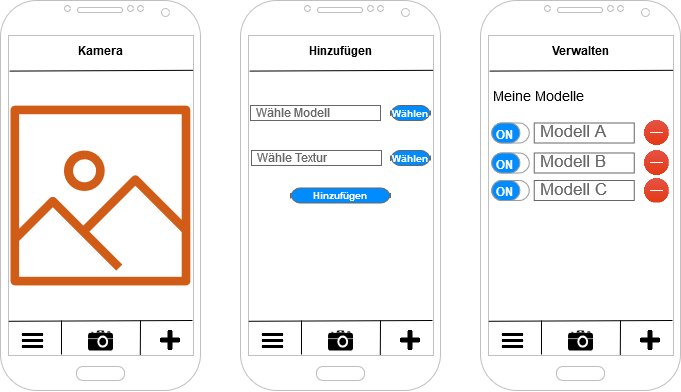
\includegraphics[width=0.8\textwidth]{Abbildungen/ui-mockup.png}
\caption[UI Mockup]{Das Mockup des User Interfaces. (Quelle: Eigene Darstellung)}
\label{fig:ui-mockup}
\end{figure}
Es zeigt die drei Ansichten (Fragments) der Anwendung, welche von der Navigation überlagert werden. \\
Die Navigation besteht aus zwei Teilen am oberen Bildschirmrand ist der Titel des aktuellen Fragments zusehen und am unteren Rand befindet sich die eigentliche Navigation. Diese besteht aus drei repräsentativen Icons, welche jeweils ein Fragment repräsentieren. Über einen Druck auf den entsprechenden Knopf erscheint die zugehörige Ansicht.\\
Das Hauptfragment stellt die Kamera dar. Hier wird das Kamerabild analysiert und mittels Augmented Reality, um die entsprechenden Objekte erweitert. Zusätzlich ist noch ein Fragment zum Hinzufügen von Modellen und eins zum Verwalten der Fragments vorgesehen.\\
Letzteres bietet dem Nutzer die Möglichkeit bestehende Modell wieder zu entfernen.

\section{Datenspeicherung}
Die Anwendung muss die Modelle, die vom Anwendner hochgeladen werden auf geeignete weise intern abspeichern.
\todo{Überlegung zur korrekten Datenspeicherung}



